\documentclass{article}
\usepackage[utf8]{inputenc}
\usepackage{todonotes}
\title{Process and Organizational Factors that Impact Requirements Engineering and Verification and Validation Alignment}
\author{Krzysztof Wnuk, Srinivasu Akkineni}
\date{April 2020}

\begin{document}

\maketitle

\section{Introduction}
\todo[inline]{WNUK: FInd where S3 is in the thesis and put it with the right reference to the paper somewhere
Also Find where S6 should be cited and cite it as graham2002requirement
See paper S7 if it is 
Where is S8 it is the delicate balance paper by Wnuk 
Where is S10 in the paper unterkalsteiner taxonomy 

}
Requirements Engineering (RE) and Verification and Validation (V\&V) are treated inseparable and should be activated as early as possible and ensure meeting customer expectations \cite{wnuk2014delicate,bjarnason2014challenges}. Weak co-ordination between RE and V\&V can lead to ineffective development, quality problems, project delays,  additional cost and effort required for removing defects, non-verifiable requirements, lower product quality, uncertain test coverage due to lack of established channels \cite{bjarnason2014challenges,graham2002requirements,sabaliauskaite2010challenges,jones2009enabling}. 

There is a substantial body of knowledge in both RE and V\&V research fields. Despite highlighting RE and V\&V alignment as a focus area for further research in RE  \cite{sabaliauskaite2010challenges} \cite{bjarnason2014challenges} \cite{cheng2007research} and calling for investigating and exploring which additional factors may influence the balance between RE and V\&V, only a handful of studies discussed the alignment between these two areas \cite{barmi2011alignment}, e.g. how to improve requirements and testing processes \cite{kukkanen2009applying}, link requirements and testing \cite{barmi2011alignment,uusitalo2008linking,watkins1994and}, define alignment practices  \cite{bjarnason2014challenges},  define roles that support the alignment  \cite{bjarnason2014challenges} \cite{sabaliauskaite2010challenges}.

Therefore, this study occupies this gap by providing a systematic and comprehensive summarize of the research area of process and organizational aspects that impact RE and V\&V alignment. The research questions investigated in this paper are as follows: 

\begin{itemize}
    \item RQ1: In what RE phases are the RE alignment practices applied? 
    \item RQ2: What RE process factors influence the alignment between RE and V\&V?
    \item RQ3: What organizational factors influence the alignment between RE and V\&V?
    \item RQ4: What are the challenges faced during the alignment between RE and V\&V?
    \item RQ4.1: What challenges can be addressed while applying RE practices?
\end{itemize}



\section{Background and Related Work}\label{BackgroundRW}
Barmi et al. identified that the majority of the research in RE and V&V alignment is on model-based testing (MBT) including various formal methods for specifying requirements and test case generation. They also identified only three empirical studies in their mapping study \cite{barmi2011alignment}. Bjarnason et al. conducted a multi case study in six companies to investigate the challenges of RE and V\&V alignment and identified 27 alignment practices. They have synthesized the results into a conceptual model based on a V-model that shows artefacts, processes and relationship between artefacts of different abstraction levels \cite{bjarnason2014challenges,sabaliauskaite2010challenges}.
In another study Bjarnason et al.,  proposed a model for alignment of RE and V&V that involves early V&V to reduce the cost and improve the quality of the requirements \cite{bjarnason2014alignment}. Unterkalmsteiner et al. proposed a definition for alignment between requirement engineering and software testing (REST).They also proposed a taxonomy that describe the methods linking RE and testing areas and processes to determine the alignment along with the emphasis of traceability during RE and V\&V alignment  \cite{unterkalmsteiner2014taxonomy}.


Damian et al. stressed that increased testing involvement during RE activities helps the alignment.  In particular, they have found the sophisticated change control process brought the functional organization and organizational responsibility together through horizontal (designers, developers, testers and documenters) and vertical (team leads, engineers, executive management and technical managers) alignment of these roles \cite{damian2005requirements}. Furthermore, Damian et al. suggested that high relations between RE activities and V\&V can accelerate waste reduction, over scoping and requirements creep, and also improve test coverage and risk management, which resulted in increasing the quality of the product and increased productivity \cite{damian2006empirical}. 

Kukkanen et al.investigated the benefits of jointly developing the RE and testing in the safety critical domain \cite{kukkanen2009applying}. They also reported that integration of requirements and testing processes by clearly mentioning requirements and testing roles, improves by connecting people and processes from RE and testing, and this can also improved by applying good practices that support connection between RE and testing. Kukkanen et al. listed change management, traceability, requirements reviews, clear roles and responsobilities as the RE and V\&V alignment practices. Moreover, linking functional requirements and software verification provides benefits for requirement management and software implementation quality and strengthens the aligning requirements and software verification \cite{post2009linking}. Other alignment practices include early tester participation, considering feature request from testers and improved interaction and communication of different roles \cite{uusitalo2008linking}.

Lower testing and maintaining costs, increased test coverage and quality in the final output of the product can be supported by establishing traceability between requirements and other development artefacts \cite{kukkanen2009applying,uusitalo2008linking,watkins1994and}. Challenges such as communication gaps, lack of training, volatility of the traced artefacts etc. related to traceability are reported  and empirically investigated from many years  \cite{bjarnason2014challenges,cleland2003event}. Unterkalmsteiner et al. mentioned that high quality traces are expensive, but their contribution can improve the alignment and it is not only solution to achieve the alignment \cite{unterkalmsteiner2014taxonomy}.

Many formal models and languages were suggested for representing requirements for model based testing (MBT) \cite{dias2007survey}. MBT struggles with practical applicability of traceability in industrial development \cite{nebut2006automatic,yue2011systematic,aichernig2014integration}. Some promising work is reported, e.g. Nebut et al. \cite{nebut2006automatic} and Hasling et al. \cite{hasling2008model} reported that applying MBT by generating test cases from UML description of requirements benefits in increasing test coverage and testing productivity. The conversion of technical requirements into a formal model could encounter some of the difficulties such as requiring special competence to produce requirements etc. \cite{nebut2006automatic}. Therefore, Yue et al. stated that additional research is needed before proposing a practical solution to this conversion of technical requirements \cite{yue2011systematic}. 

Automated test case generation of test cases generation has the potential of linking requirements without any creation or maintenance  of manual traces  \cite{bjarnason2014challenges}. However, the value of the traces may vary by depending on the generated test cases and the abstraction level of the formal model  \cite{sabaliauskaite2010challenges}. While applying MBT, error causes in these formal models are the main hindrance to fully trust them \cite{hasling2008model,ferguson2006empirical}. As an alternative to formal models scenario-based models are defined such as user stories, use cases \cite{regnell2000towards,regnell1998combining}  to cover requirements. In scenario based models acceptance test cases are used to document the detailed requirements at a high level and this approach is often applied in agile development by Cao and Ramesh \cite{cao2008agile}. In  another study Melnik et al. found that to implement and feather testing mentality, executable acceptance test cases can be used as detailed requirements \cite{melnik2006executable}.

Process factors, contextual factors and organizational factors play an important role in the alignment. Bjarnason et al. discussed the consideration of process factors i.e. source of requirements, requirements in typical project \cite{bjarnason2015industrial}. In a similar study to this, Kukkanen et al. stressed to know the importance of process factors which may shorten the development time and improve the quality \cite{kukkanen2009applying}. Sabaliauskaite et al.  discussed the influence of organizational factors i.e. organizational structure, gaps in communication across different organizational units, however without details \cite{sabaliauskaite2010challenges}.  Bjarnason et al. discussed influence of organizational factors during a study to present an initial version of a theory based on the GAP model \cite{bjarnason2013distances}. During this study they have discussed the organizational factors that influence the alignment i.e. size of an organization, domain and range of an organization. Whereas, Wnuk et al.  discussed the impact of enabling factors such as focus on informal and direct communication, open culture for the success of a software project \cite{wnuk2014delicate}.

\section{Research Methodology}\label{RM}


We have used a snowballing method for searching the relevant literature \cite{wohlin2014guidelines}. The reason for not choosing the database search, e.g. SLR is because it is quite difficult to formulate a precise search string due to different terminology that increases the number of irrelevant papers in the search \cite{wohlin2014guidelines,kitchenham2009systematic,kitchenham2010systematic}. Moreover, snowballing can also be used as a reference for identification of additional list of studies through citations and references of selected studies \cite{wohlin2014guidelines} or for extending previous systematic literature reviews, e.g. Bjarnason et al. \cite{bjarnason2013distances} or Barmi et al. \cite{barmi2011alignment}.

\subsection{Start set selection }
We selected the “Engineering village” database for start set identification. Google scholar was excluded as it lacks in providing certainty in terms of scholarly value and currency of some records, lacks in including the scope of its coverage. As suggested by Kinsely et al.,  Engineering Village is an appropriate place to initiate an engineering search when compared to other databases \cite{knisely2014engineering}. 

The search string used for start set identification was iteratively developed with intensive discussions between the authors. Some categories were derived from the research questions and based on the study of initial set of papers.  These categories focus on Non-functional requirements (F1), Requirements (F2), verification and validation (F3) and alignment(F4). Search string formulated by using these categories is “F1 OR F2 AND F3 AND F4”. 
\begin{itemize}
    \item  F1: "nonfunctional requirement" OR "nonfunctional requirements" OR "non functional requirement" OR "non functional requirements" OR "non functional software requirement" OR "non functional software requirements" OR "nonbehavioral requirement" OR "nonbehavioral requirements" OR "non behavioral requirement" OR "non behavioral requirements" OR "non behavioural requirement" OR "non behavioural requirements" OR "nonfunctional property" OR "nonfunctional properties" OR "non functional property" OR "non functional properties" OR "quality attribute" OR "quality attributes" OR "quality requirement" OR "quality requirements" OR "quality attribute requirement"
    \item F2: “Requirements” 
    \item F3: "test" OR "tests" OR "testing" OR "verify" OR "verifying" OR "verification" OR "validate" OR "validation"
    \item F4: "align" OR "aligning" OR "alignment" OR "trace" OR "tracing" OR "traceable" 
\end{itemize}





The above search string covers the entire alignment between RE and V\&V unlike just RE practices, RE process factors, organizational factors and challenges faced during alignment between RE and V\&V. The idea here was to capture the verification and validation practices along with RE practices that are followed during the RE and V\&V alignment. We decided to look for papers from 2001 or younger following the recommendation of Barmi et al. who mentioned that research on alignment between RE and testing was started from the end of year 2001 \cite{barmi2011alignment}.

Start set was derived by:
\begin{itemize}
    \item Extraction of studies from database using a search string: 5787 papers were identified.
    \item By considering the papers between 2002 to 2019, we identified 4202 paper candidates.
    \item By screening considering the inclusion and exclusion criteria, we ended up in with 690 potential papers.
    \item From these 690 results by examining the abstract and further screening 658 papers were not found relevant and therefore excluded. The remaining 32 candidates were considered as a tentative start set.
    \item After performing full text read, we included 10 papers from the 32 candidates. We investigated the diversity of the 10 paper candidates with an aim for achieving the possibility of more coverage of relevant studies \cite{wohlin2014guidelines}. These 10 papers were considered as a start set. 
\end{itemize}
The inclusion criteria included:
\begin{itemize}
    \item IC1: Studies must be available in full text.
    \item IC2: Studies must be available in English language.
    \item IC3: Studies should be peer reviewed.
    \item IC4: Studies that have any type of alignment related to requirements and   V\&V should be included.
    \item IC5: Studies related to formal methods, software engineering techniques and Diagnostic, testing and debugging method classification codes are included.
    \item IC6: Conferences, journals, articles that are published in between 2002-2019 years are included.
    \item IC7: Process and organizational factors influencing the alignment 
    \item IC8: The study that reports the benefits, challenges, disadvantages, practices of alignment.

\end{itemize}

\textbf{Data extraction and synthesis:} Data extraction properties were created in spreadsheets and also mapped with research questions before finalization. The data extraction properties included: 

General information (Authors, Title, Year of publication, Abstract), Study type (Proposal of solution Evaluation research, Validation research Philosophical papers, Opinion papers
Personal experience papers), Research method used (Case study,  Experiment,  Survey ,  Framework), Research problem (i. Does the study specify the RE practices during alignment between RE and V\&V? ii.	Does the study specify the specific RE process factors? iii.	Does the study specify the specific organizational factors? iv.	Does the study specify the challenges that are faced during the alignment between RE and V\&V?), Outcomes (i.	Practices during alignment between RE and V\&V, ii.	Influence of factors, iii.	Challenges).


Rigor and relevance criteria were used to check the trustworthiness of each paper, according to the checklist provided by Ivarsson et.al \cite{ivarsson2011method}. This helps in identifying weather the results are suitable for the identification of practices, challenges and influencing factors in alignment study.


\textbf{Synthesis:} We used narrative analysis for analyzing the results obtained through literature, narrative. Narrative analysis is defined as “an approach to the systematic review and synthesis of findings from multiple studies that relies primarily on the use of words and text to summarize and explain findings of the synthesis”. This approach helps in process of explaining the data retrieved from the identified studies in a ‘tell the story’ way. This also used to synthesis the data that can be used in the identified studies, which were focused on a wide range of research questions, not only studies related to the effectiveness of a particular research area \cite{popay2006guidance}.


\subsection{Validity}


\textbf{Construct validity:} threats refer to the information relevant to alignment between RE and V\&V and the presence of confounding factors whether or not this study capable to capture its aims and objectives. Construct validity threats are reduced by detailing the section and planning according to the formulated research questions. One of the main threats for using snowballing approach for SLR is obtaining a good start set. Using the guidelines suggested by Wohlin \cite{wohlin2014guidelines} for obtaining a good start set such as, design of start set is extended with the change in database selection is followed. This mitigates the risk of obtaining irrelevant studies. Moreover, to mitigate the risk of resulting same author, some authors were excluded during the selection of start set of papers. Finally, the thesis supervisor was involved in the start set selection and snowballing iterations to ensure that the inclusion decisions are fully justified and uncertainties are resolved.

\textbf{Internal validity:} Since the authors did the selection of the studies, internal validity is one of the major challenges. Selection bias is mitigated by being broad as possible and discussing the uncertainties between the two authors. By strictly following the guidelines for snowballing procedure and for quality assessment criteria, the internal validity for this study is enhanced. 

\textbf{External validity:} To increase external validity, the start set was composed from a database search with Engineering Village selected as a source that has a broad range of engineering conference and journal publications. The use of snowballing method for searching articles helps to mitigate external validity threats. 

\textbf{Reliability:} threats are mitigated by analyzing four studies related to alignment between RE and V\&V (that were included in start set) to verify the accuracy and the strength of search string. However, this benefits in minimizing the selection bias, which might have impact on further steps of this research.  Furthermore, backward and forward snowballing was carried out and resulted in attaining relevant studies of RE and V\&V alignment. Moreover, the thesis supervisor was involved in the start set selection and snowballing iterations to ensure that the inclusion decisions are fully justified and uncertainties are resolved.
The data extraction properties were reviewed by the both authors. Moreover, quality of the identified studies is an important objective since this research focuses on factors and practices related to industry. Therefore, quality assessment is carried out by applying the rigor and relevance assessment criteria suggested by Ivarsson and Gorschek \cite{ivarsson2011method}. 

\section{Results and Analysis}\label{ResultsAndAnalysis}

\todo[inline]{WNUK: start here with editing 
CHECK THe citations of papers S1 to S20 from 2016 to 2019 and update the number of citations screened in the table below, check if there is any new paper or not, 

Also list the start set S1, S2 .. with the references
Fix the }

\begin{table}[]
    
    \hline
    \begin{tabular}{|p{1.5cm}|p{2.5cm}|p{2.5cm}|p{2cm}|p{2cm}|}
   
         &  Backward (evaluated and included studies) & Backward removed (what and why) & Forward (evaluated and included) & Forward removed (what and why) \\
          \hline
       First iteration  &  280:4 \newline (S11\cite{metsa2007testing}, S12\cite{bjarnason2015industrial}, S15\cite{ferguson2006empirical}, S16\cite{bjarnason2014alignment}) & 56-Pub. year, 22-Pub. type, 153-Title
53-Abstract and full text & 237:2 \newline (S13\cite{aichernig2014integration}, S14\cite{bjarnason2015industrial}) & 101-Title 29-Language 38- Duplicates 66- Full text and abstract \\
\hline
Second Iteration & 124: 2( S17 \cite{melnik2006executable}, S18 \cite{bjarnason2013distances}) & 33- Publication Year 11- Duplicates 9- Language 23- Title 2-Full text & abstract & 39:0 & 9- Language 23- Title 4- Duplicates 2-Full text and abstract \\
Third iteration & 69:0 & 17- Publication Year 37- Title 2- Duplicates 13- Full text and abstract & 44: 2(S19 \cite{melnik2004suitability}, S20) & 26- Title 6- Language 4- Duplicates 8-Full text & abstract \\
Fourth Iteration & 20:0 & 12- Publication year 6- Title and abstract 2- Full text & 43:0 & 26- Title 4- Duplicates 6- Language 6-Full text and abstract \\
\hline
    \end{tabular}
    \caption{Caption}
    \label{tab:my_label}
\end{table}

\subsection{Categorization based on the study type and research method}\label{ResultsCat}

The results were categorized into the two methodological dimensions, based on the suggestions given by Runeson et al.[42] and Wierlinga et al. [43], namely methodology (Survey, case study, tool proposal and framework) and type of study (proposal, evaluative, validation and solution). Figure 2 depicts the categorization of these two dimensions. 

12 studies (S3, S4, S8, S9, S10, \cite{lobo2005local}, \cite{aichernig2014integration}, \cite{ferguson2006empirical}, \cite{bjarnason2014alignment}, \cite{melnik2006executable}, \cite{bjarnason2013distances}, \cite{melnik2004suitability}) were considered as evolution research, two studies were categorized as solution studies (\cite{ricca2007talking}, S2) and three studies proposed a framework for aligning test cases with requirements (S7, \cite{metsa2007testing}, \cite{bjarnason2015industrial}). We considered studies S2 and \cite{ferguson2006empirical} as secondary studies and study S6 is an opinion paper.  
 
The majority of the identified studies rapport evaluation research should enable finding the practices that improve RE and V&V alignment. However, the identified papers seem to primarily focus on descriptive studies that describe the RE and V&V misalignment cases rather than how to improve the alignment [11].
Evaluations using case study research methodology dominates among the identified papers. Three studies were classified as case study-solutions, one paper was classified as validation research and one as a proposal.  Two out of four (\cite{ferguson2006empirical}, S17, \cite{melnik2004suitability}, S20 \cite{ricca2007talking}) studies reported evolutions using experiments performed with students as subjects. It remains to be determined if students are representative population for studying alignment issues. On the other hand, four studies performed non-experimental evaluations (S2, S5, S9, \cite{bjarnason2014alignment}) and suggested the practices that strengthen RE and V&V alignment.
Finally, framework-solution and framework-proposal received only 1 study each. No studies were found in survey, experimentation-proposal, solution and also in framework-validation, evolution categories. 
The much higher number of identified case studies compared to experiments implies that conducting experiments in the context of alignment between RE and V&V is challenging because of the difficulty in operationalizing the alignment practices into the set of measurable independent variables. The other challenge is how to identify the causality in this study as there could be several confounding factors that influence the alignment between RE and V&V.

\begin{figure}
    \centering
    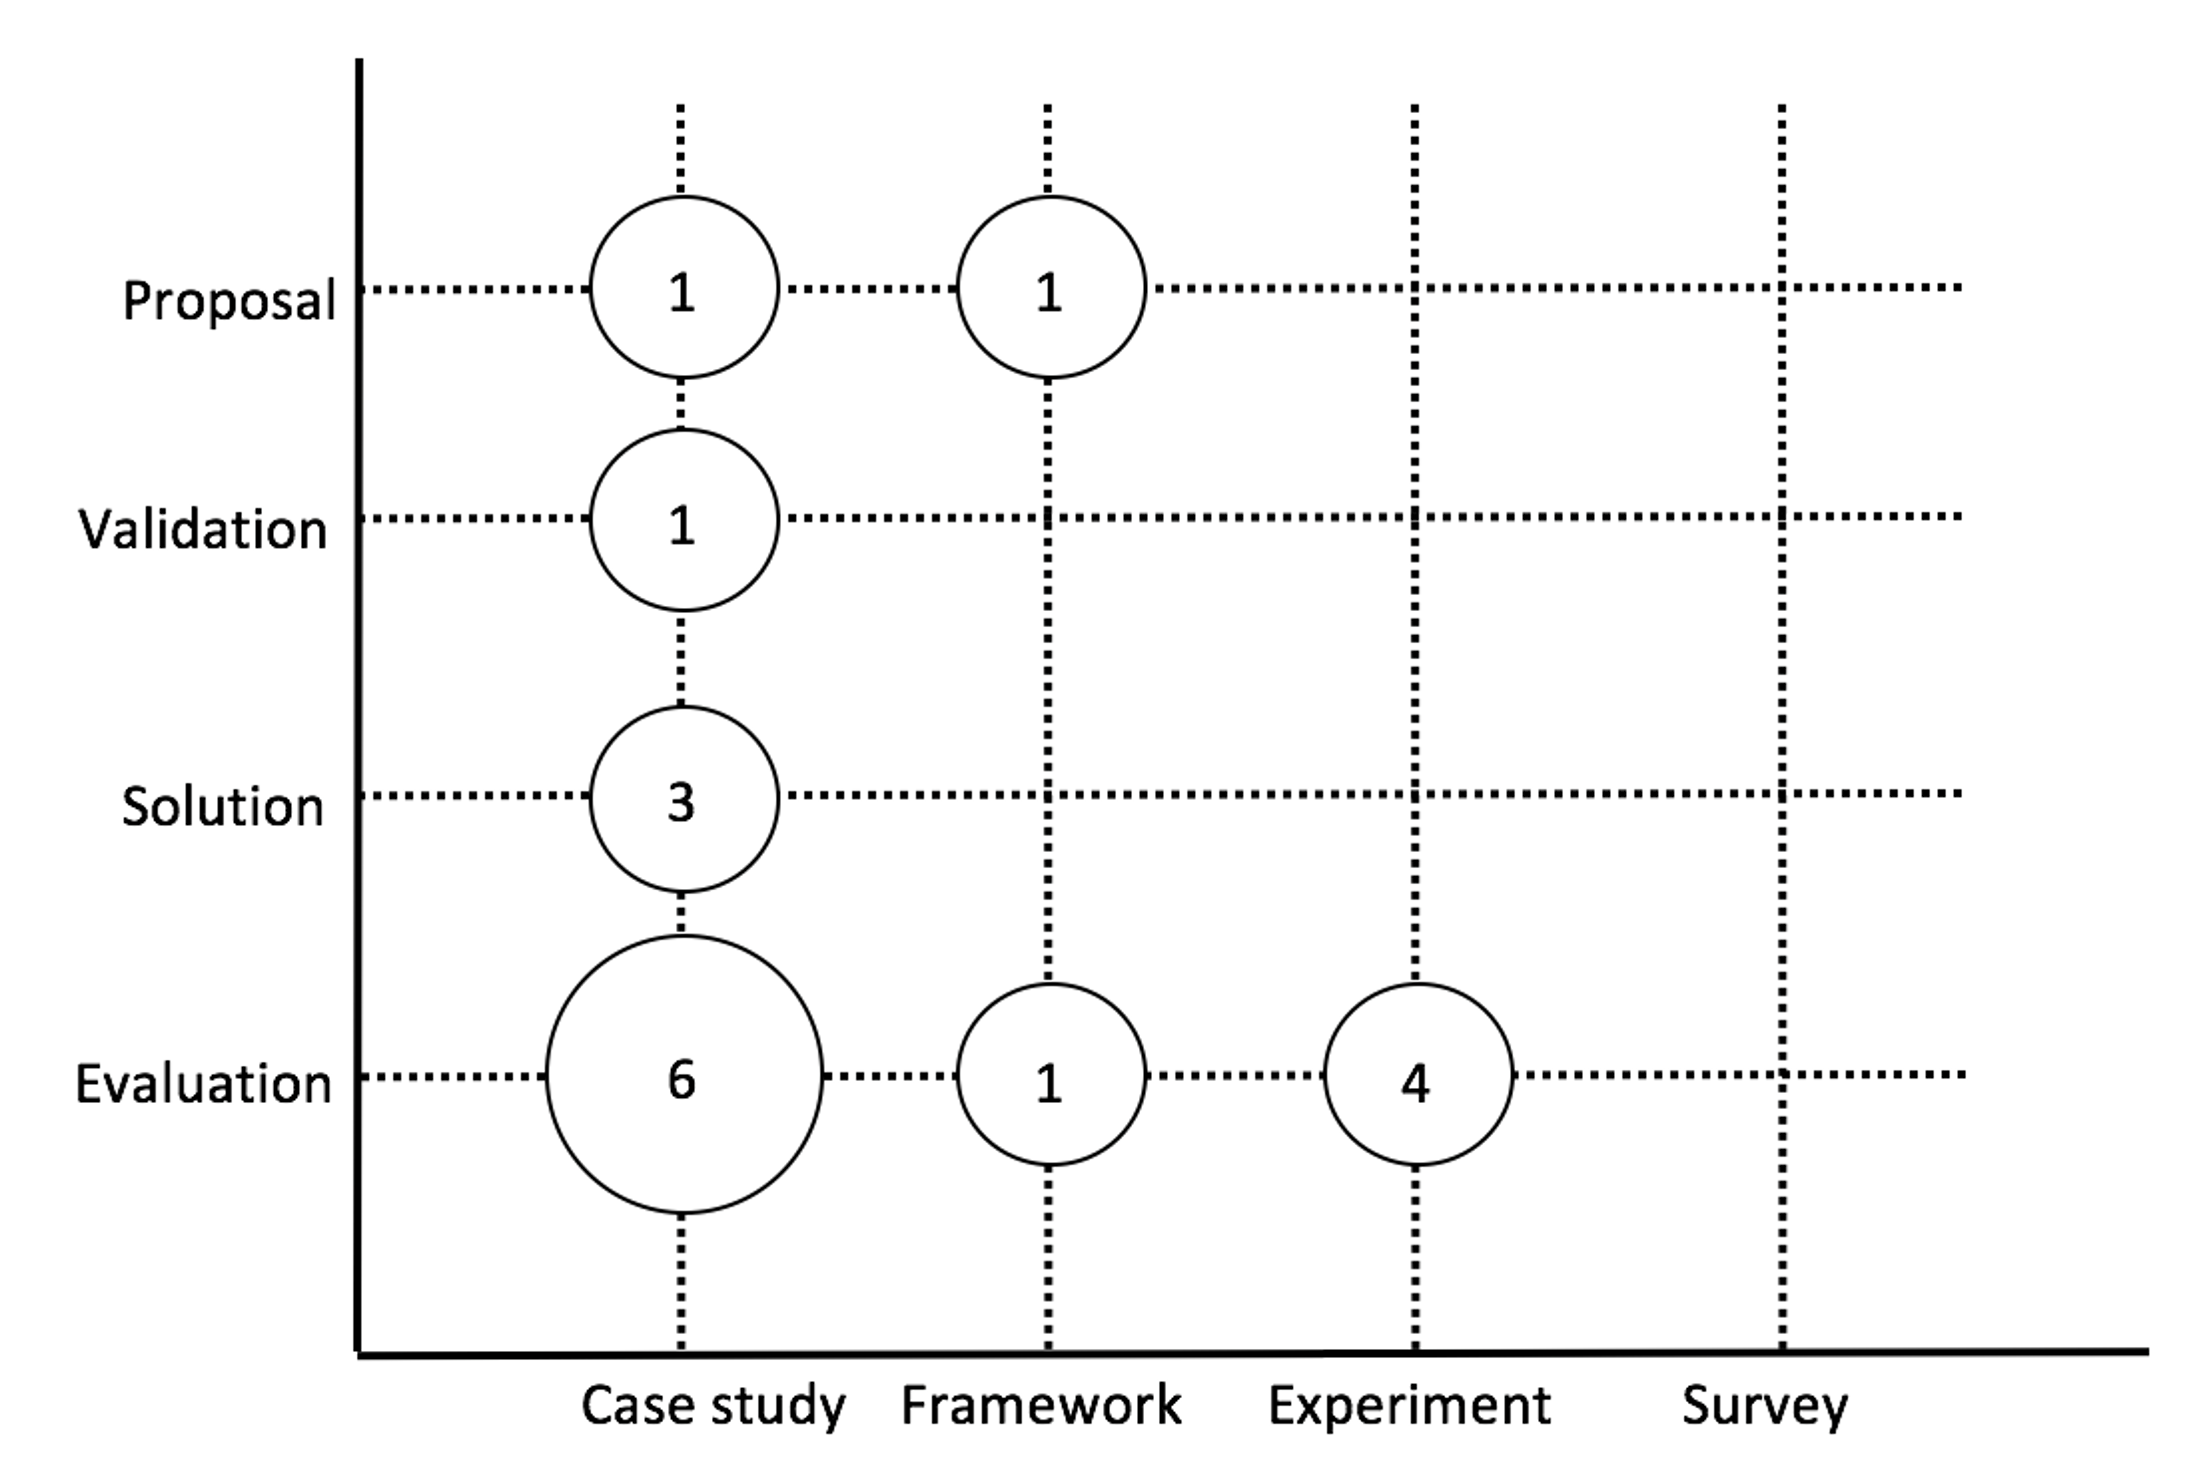
\includegraphics[width=\textwidth]{Classification.png}
    \caption{Classification of the studies based on the study type and research method.}
    \label{fig:my_label}
\end{figure}

\subsection{Quality assessment based on rigor and relevance}\label{RigorAndRelevance}

8 studies (S2, S4, S7, S5, S3, S9, \cite{bjarnason2014alignment}, S10) are classified as having highest rigor and relevance, see area A in Figure 3 and these are the most trustworthy results. Moreover, 5 studies (S8, \cite{metsa2007testing}, \cite{lobo2005local}, \cite{bjarnason2015industrial}, \cite{ferguson2006empirical}) are classified in the B category with high relevance but low rigor. On the other hand, 4 studies are classified in the C category as they represent low relevance and low rigor, see area C in Figure 3 and no studies were identified with high rigor and low relevance, see area B in Figure 3. The rigor and relevance scores for the identified studies are attached in Appendix B. 
Evaluation of rigor and relevance scores for the identified studies resembles the usage of rubric based evaluation in education system [40]. This evaluation of rubrics helps to increase the reliability of assessments in the form of inter-rater agreement between researchers. 
It is interesting to mention that the identified case studies have higher rigor and relevant scores than the experiments. A possible explanation for this may be that the experiments were not carried out in the industrial setting, unlike the case studies. Most of the identified studies with higher rigor relevance describe the RE practices, RE process factors, organizational factors and challenges during the alignment between RE and V&V, which were relevant to this research study. 

\begin{figure}
    \centering
    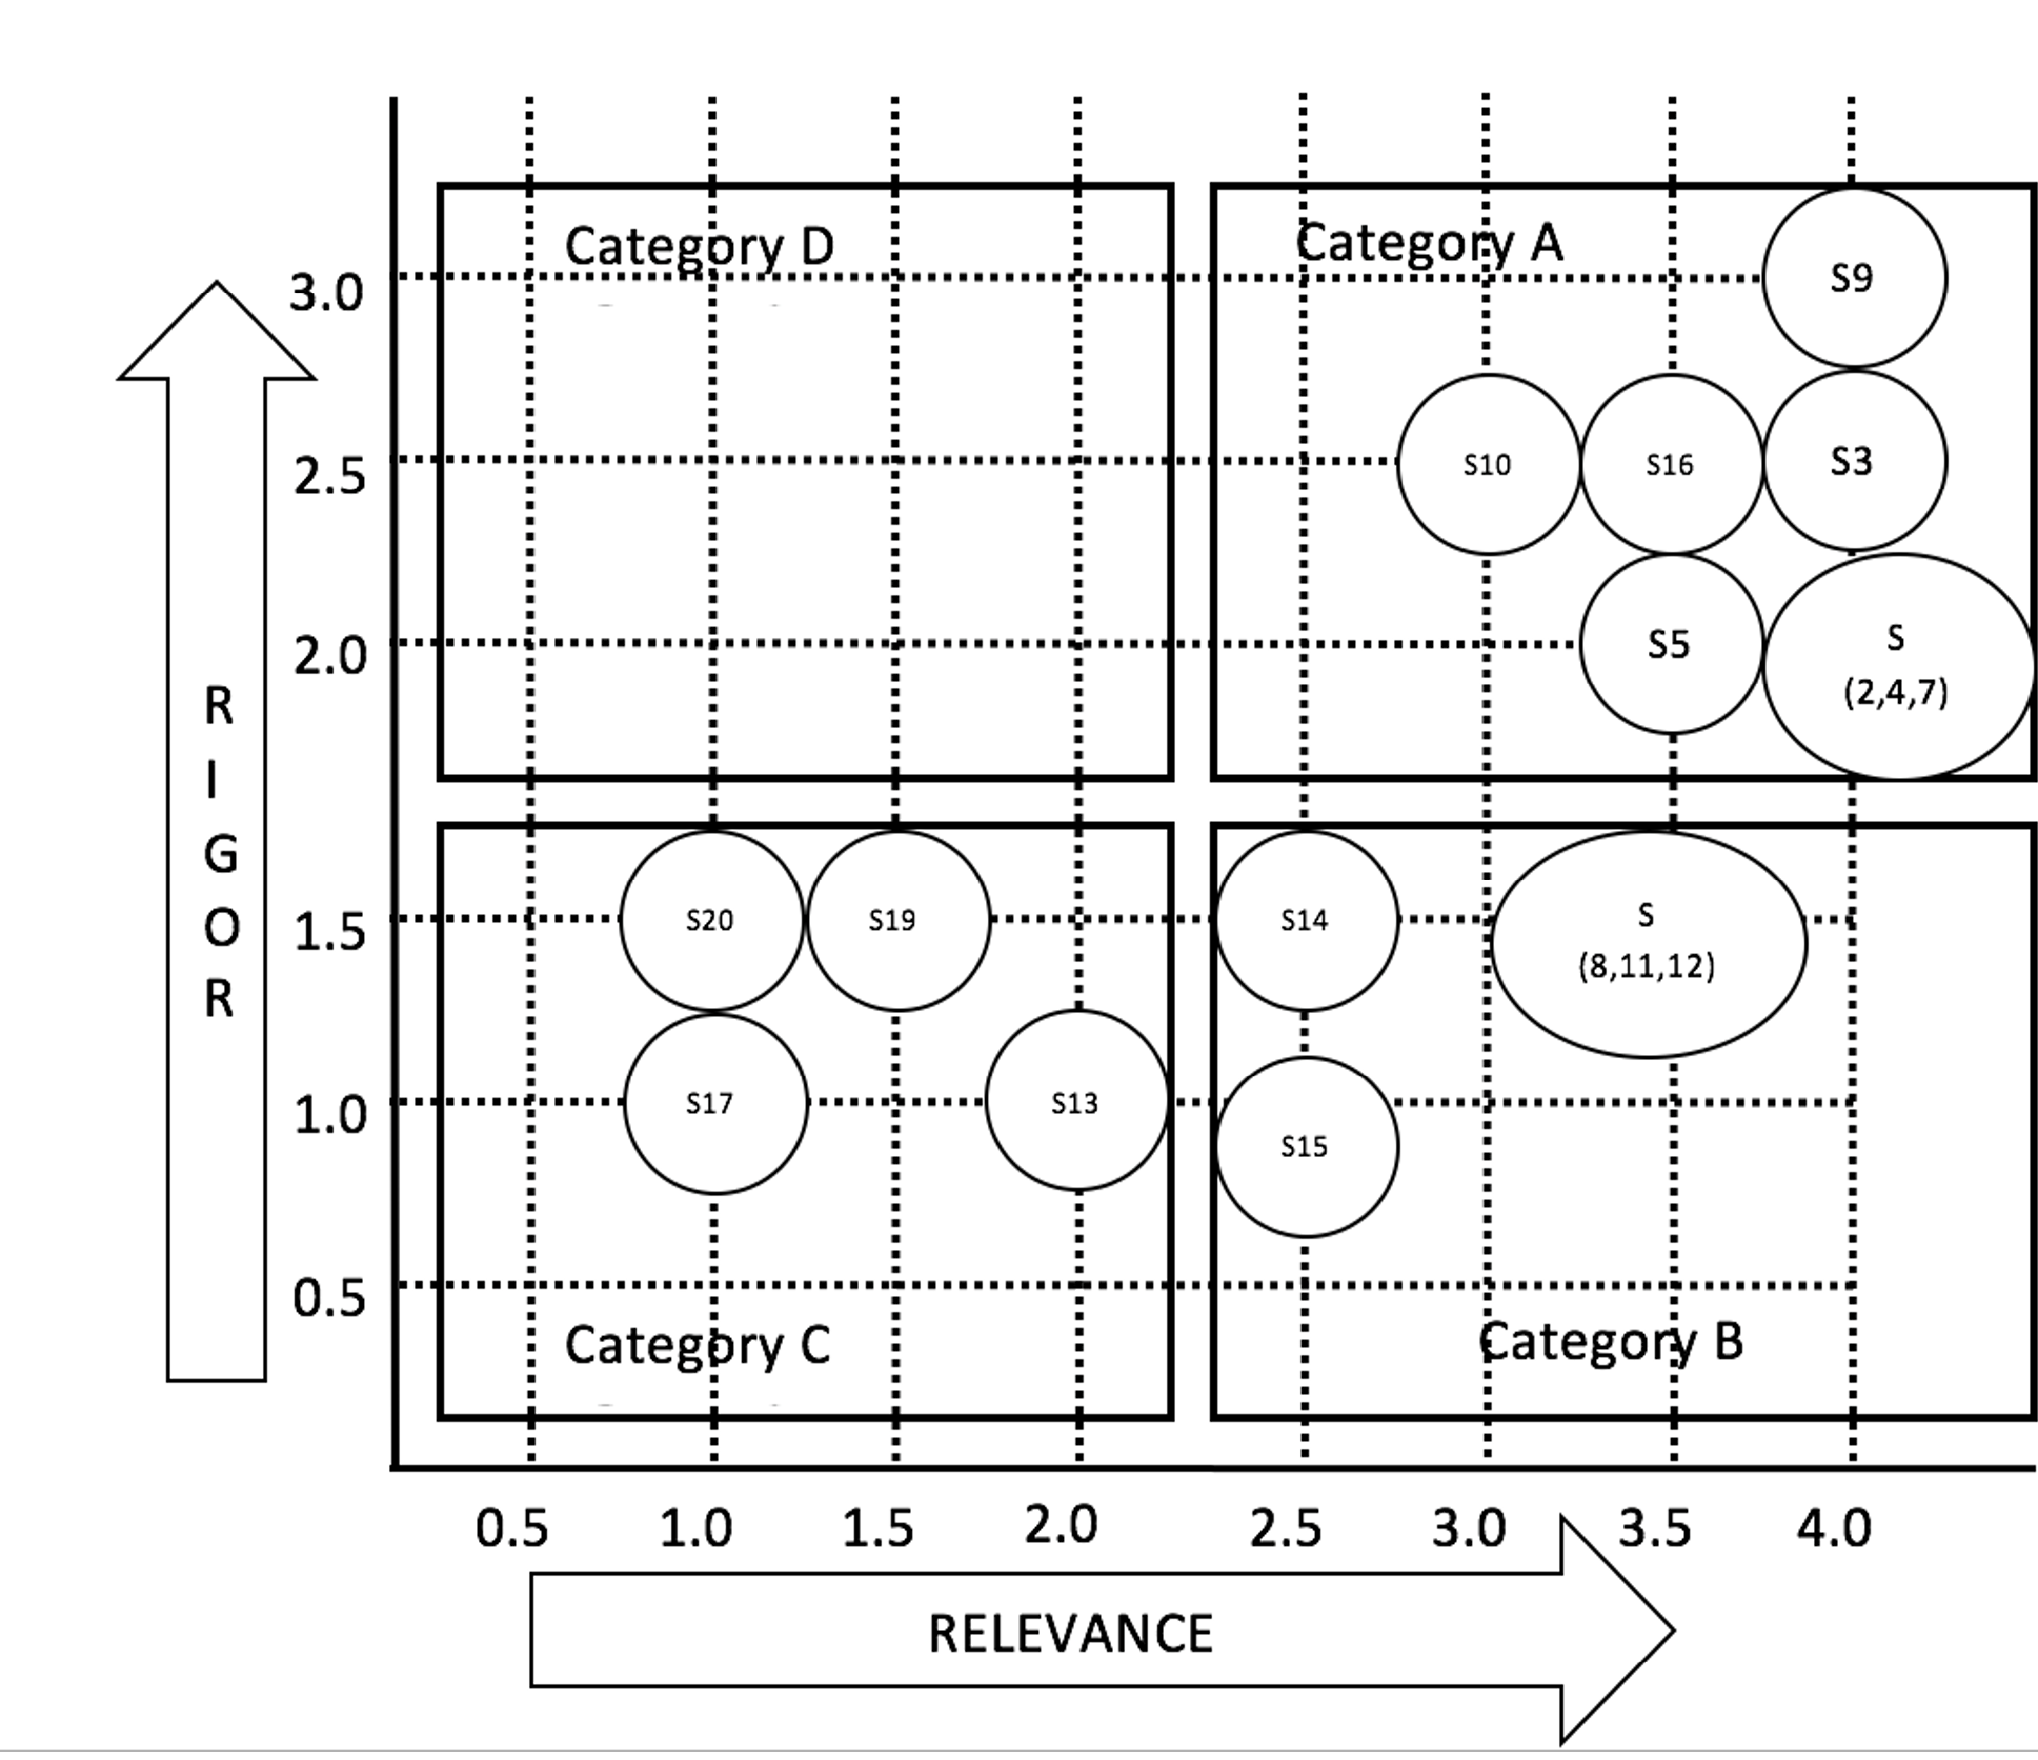
\includegraphics[width=\textwidth]{RigorAndRelevance.png}
    \caption{Rigor and Relevance Analysis}
    \label{fig:my_label}
\end{figure}

\subsection{Quality Assessment criteria for secondary studies}

Quality assessment for secondary studies should be performed in order to minimize the bias and maximize the internal and external validity of the study[44]. The quality criteria such as specification of methodology, specification of clear results etc. and scale of measurement (Yes, Partially, No) are presented in appendix C. \todo[inline]{WNUK: Fix appendix C}

\subsection{RE practices during the alignment}\label{ResultsPracticesDuringAllignment}

In this section the analysis of primary studies is carried out regarding the RE practices that are used while improving the RE and V\&V alignment. 
Six studies \cite{barmi2011alignment} \cite{kukkanen2009applying} \cite{uusitalo2008linking} \cite{bjarnason2014challenges} [\cite{bjarnason2015industrial}] [\cite{bjarnason2014alignment}] discussed different practices that are used during the alignment of RE and V\&V. From the Figure 3 it can be observed that most of these studies (\cite{kukkanen2009applying} \cite{uusitalo2008linking} \cite{bjarnason2014challenges} [\cite{bjarnason2014alignment}]) have high rigor and relevance. Uusitalo et al.[11] (S[5]) Performed an interview study to identify practices that are used for strengthening the alignment between RE and testing. This study has primarily concentrated on identification of practices used for strengthening the link between RE and testing and has also identified the challenges, benefits during application of these practices. During their study some of the interviewee considered linking people and linking documents are essential for alignment of RE and testing. Similar practice is also suggested in a case study conducted by Kukkanen et al. [10] (S2\cite{bjarnason2014challenges}) in order to identify the set of good practices that helps the concurrent improvement of RE and testing processes.  They also discuss the roles and their main responsibilities that are need to link requirements and testing. This case study results implies that, it is important to perform linking in three levels 1) linking processes 2) linking of people and 3) applying good practices along with linking of people and documents.

Thereafter, Barmi et al. (\cite{barmi2011alignment}) has performed a systematic mapping study on alignment of requirements specification and testing. They identified the studies that discuss on linking specification and testing of requirements. They primarily focused on problems and set of good practices in aligning the requirements and testing. Similar practices are also discussed in a case study performed by Bjarnason et al.[33] (S[14]) to identify the scenarios for applying the alignment practices. These findings also includes benefits and challenges in using test cases for validating, eliciting, tracing, verifying and managing requirements. Overall, this case study provide how the discussed practices meet the requirement roles at different stages.

Thereafter, in a multi case study of six companies Bjarnason et al. \cite{bjarnason2014challenges} (S[9]) has identified 27 different alignment practices, grouped into 10 categories. They also discuss challenges faced while application of practices such as cross role requirements reviews, product manager review types, early verification start, document level traces, test cases as requirements, traceability responsibility role, independent testing etc. These challenges are namely V\&V quality, full test coverage, verifying quality requirements etc. are mapped with the 27 alignment practices. These findings help practitioners and researchers for recognizing challenges faced and practices applied to address these challenges during the alignment between RE and V\&V.  

In another study Bjarnason et al.[34] (S[16])discuss alignment practices that affect the distances in software development. And some of the studies S [14] have not mentioned about impact of the identified practices during the alignment.

The practices considered while applying alignment between RE and V\&V are \cite{barmi2011alignment} \cite{kukkanen2009applying} \cite{uusitalo2008linking} \cite{bjarnason2014challenges} [\cite{bjarnason2015industrial}] [\cite{bjarnason2014alignment}] presented in Appendix D. As mentioned previously these aspects cover the practices that are used during the alignment of requirements and testing. These practices are needed for an organization in to order to achieve the RE and V\&V alignment. This constitutes to the identification of the RE practices that are used during the alignment of RE and V\&V S[9], S[16], S\cite{bjarnason2014challenges}, S[5]. The obtained literature is analyzed in order to identify RE practices used in specific to requirement phases. Identified RE practices through literature are mentioned and discussed below.

RE practices are at the core of aligning the RE and V\&V\cite{bjarnason2014challenges}. These practices include involving development near roles, informal communication within organization and customer communication in the requirement process.

\begin{itemize}
    \item \textbf{Customer communication at all levels and in all phases of development (S9\_1, \cite{bjarnason2014alignment}\_18)}: Communication can be made in the mode of customer-supplier for co-location, customer based interaction used for demonstrating executable software or agreed acceptance criteria between customer and supplier \cite{bjarnason2014challenges}.For smaller companies with bespoke requirements interaction is directly with a physical customer. Whereas, in larger companies customer proxy is used instead of real customer for the interaction \cite{bjarnason2014challenges}. In each development team a person should take responsibility for the feature scope. However, that person should be available to communicate throughout the development and the validation of particular feature \cite{bjarnason2014challenges}. Therefore, this practice should be carried out all requirements phases to ensure the communication with customers.
    \item \textbf{Involving developers and testers in detailing requirements (S9\_2,  \cite{bjarnason2014alignment}\_19): }
    This practice is considered as a deliberate strategy for conveying the main goal of the product to the engineers rather than detailing requirements. Here development organization will take the responsibility of detailing the specification. This may be considered as a risky practice if there is a weak awareness of the market perspectives or customers \cite{bjarnason2014challenges}. This practice also consist of involving testers at the early stages of the entire project[11]. This benefits in improving the testers gaining knowledge on domain\cite{bjarnason2014challenges}. 
    \item \textbf{Cross role requirement reviews (S9\_3, \cite{bjarnason2014alignment}\_20)} : This practice is applied to ensure that requirements are understood and testable. The practical procedures for the review of requirements are namely early review of requirements by testers and reviewing the requirements while creating test cases. Furthermore, this practice enhances both quality of requirements and communication resulting in strengthening the alignment of the testing effort. Therefore, this practice helps in identifying problems with the test specification at early stages \cite{bjarnason2014challenges}. 
    \item \textbf{Defining a requirements review responsible (S9\_4):} Kukkanen et al. [10] discovered the role of assurance manager overlaps with test and requirement manager roles. They stress the importance of an additional responsible role for requirement reviews. Hence, defining a requirement review responsible was mentioned as a practice \cite{bjarnason2014challenges}. This ensures that requirement reviews are performed. This role is decided during the requirement analysis phase.
    
    \item \textbf{Involving domain experts in requirement definition (S9\_5):} This practice is applied to achieve better co-ordination between system capabilities and requirements. This leads to defining more realistic requirements \cite{bjarnason2014challenges}. By applying this practice, domain experts will know if they understand the requirement correctly or not \cite{bjarnason2014challenges}. This practice also considered for supporting the alignment by improving the quality of requirements, which were the basis for software testing.
    
    \item \textbf{Documentation of requirement decision rationales (S9\_6):} This practice increases the synchronization between different project phases by supporting transfer of soft communication between different roles S[2]. After completion of development, this information will support testers in evaluating customer defect reports and in identifying required improvements. However, this information should be easily connected and available to the test cases and requirements for the use of testers in later stage of development \cite{bjarnason2014challenges}.

\end{itemize}


The above mentioned RE practices are discussed in literature that influences the alignment between RE and V\&V. These practices will create positive effect on RE and V\&V alignment\cite{bjarnason2014challenges}[10][11][15].Whereas, Bjarnason et al. has discussed about the additional practices that were identified through the analysis performed for constructing the GAP model[34]. Following are the identified RE practices used for RE and Testing (RET) alignment by Bjarnason et al [34].

\begin{itemize}
\item 	Use of customer proxy role (\cite{bjarnason2014alignment}\_1).
\item 	Feature requirement documentation (\cite{bjarnason2014alignment}\_2).
\item 	Product manager physically present to developers \& testers (\cite{bjarnason2014alignment}\_3).
\item 	Informal communication with in organization (\cite{bjarnason2014alignment}\_4).
\item 	Same processes for quality requirements(\cite{bjarnason2014alignment}\_6).
\item 	Structure requirement artefacts accord to type (\cite{bjarnason2014alignment}\_7).
\item 	Collaborative definition of quality requirements (Quality requirements, e.g. performance, usability etc.). (\cite{bjarnason2014alignment}\_8).
\end{itemize}

 Bjarnason et al. [34] mentioned about the additional identified practices. However, they have not discussed their impact on the study of alignment. They primarily focused on how these practices are showing impact on distances i.e. geographical distance, organizational distance, cognitive distance. In specific, they discussed how two RE practices (i.e. product manager physically present to developers \& testers, collaborative definition of quality requirements) impact the distances.

It is important to notice that some practices such as requirements test case traces, same abstraction levels for requirement specifications are not considered as RE practices. This is due to fact that Bjarnason et al.\cite{bjarnason2014challenges}, have simplified the view of RE and V\&V alignment, by considering traceability activities to be different from RE practices. Therefore, in this study we considered only RE practices without traceability practices as suggested by Bjarnason et al. \cite{bjarnason2014challenges}. 



Table  \ref{tab:RePractices} presents the list of all identified RE practices used during the alignment and their usage at different requirement phases.

\begin{table}
    \centering
    \begin{tabular}{|p{1cm}|p{5cm}|p{1cm}|p{1cm}|p{1cm}|p{1cm}|}
    \hline
         ID & Description & Elicita tion & Anal ysis & Speci fication & Vali dation \\
            \hline
         P1 & Customer communication at all levels and in all phases of development (S9\_1)  (\cite{bjarnason2014alignment}\_18) & X & X & X & X \\
          \hline
         P2 & Involving developers and testers in detailing requirements (S9\_2) (\cite{bjarnason2014alignment}\_19) & & & X & \\
          \hline
        P3 & Cross role requirement reviews (S9\_3)  (\cite{bjarnason2014alignment}\_20) &  & X & &  \\
         \hline
        P4 & Requirements review responsibilities defined (S9\_4) & & X & &  \\
         \hline
        P5 & Subsystem expert involved in requirements definition (S9\_5) & X & & &  \\
         \hline
        P6 & Documentation of requirements decision rationales (S9\_6) &   & X & & \\
         \hline
         P7 & Use of a customer proxy role (\cite{bjarnason2014alignment}\_1) & X &  & &  \\ \hline 
         P8 & Feature requirements documentation (\cite{bjarnason2014alignment}\_2) &  & & X &     \\ \hline
         P9 & Informal communication within organization (\cite{bjarnason2014alignment}\_4) & X & X & X & X \\ \hline
         P10 & Same process for quality requirements (\cite{bjarnason2014alignment}\_6) & X & X & X & X \\ \hline
         P11 & Structure requirement artefacts accord to type (\cite{bjarnason2014alignment}\_7) &  & & X & \\ \hline
         P12 & Collaborative definition of quality requirements. (\cite{bjarnason2014alignment}\_18) & X & & &  \\ \hline
    \end{tabular} 
    \caption{Applying alignment practices at different requirement phases}
    \label{tab:RePractices}
\end{table}

Many of these RE practices namely customer communication at all requirement levels & phases, informal communication with in organization, same process for quality requirements, product manager physically present to developers & testers should carried out through all the requirement phases[28]. Development involved in detailing requirements and documentation of requirement decision rationale practices are considered in both requirement analysis and specification phases. It is done more during the requirement specification phase. Feature requirements documentation is another practice that is involved in the specification and analysis phase. This practice is considered to ensure that requirements are actually analyzed and defined on feature level instead of all possible levels. The use of a customer proxy role and collaborative definition of quality requirements practices are considered during requirement elicitation and analysis phases, however more intensively in the requirement specification phase.

\subsection{Analysis of literature regarding RE process factors during the alignment}\label{ResultsProcessFactors}

Primary studies were also analyzed in order to identify the influence of various RE process factors during the alignment. Identification of the impact of RE process factors while implementing practices is one of the areas in this research. 
Many of the authors have tried to provide influence of RE process factors during the alignment. Sabaliauskaite et al.  mentioned the influence of RE process factors i.e. source of requirements, however without deeper analysis. The emphasis was made on identifying the challenges rather than influence of process factors on the alignment. Similarly, Bjarnason et al. [33] discussed the process factors, while performing a case study to find the benefits and challenges in using test cases for elicitation, validating, verifying, tracing and managing requirements. During this study they have discussed the consideration of process factors i.e. source of requirements, requirements in typical project. In a similar study to this, Kukkanen et al.[10] stressed to know the importance of factors which may shorten the development time and improve the quality. In another study\cite{bjarnason2014challenges}, Bjarnason et al. also considered several process factors while applying different alignment practices. They mainly focused on discussing the challenges faced while applying the identified set of alignment practices along with some process factors. Similarly, the studies [34]\cite{wnuk2014delicate} have reported influence of the RE process factors while applying the alignment practices. 
\begin{itemize}
    \item Distance between development of requirements and testing: Sometimes, development units and testing units will not give enough attention and consideration to the requirements [6][45]. During development developers do not always review requirements and this might be due to lack of involvement of testers and developers in requirement reviews[6].
    \item Testability of requirements: Testability of the requirements is not considered by the requirement engineers. This leads in turning out requirements to be non-testable [6]. Therefore, this might show negative impact on the alignment. 
    \item	Source of requirements: Source of requirements can be market driven and bespoke. However, some organizations with more number of requirements will use both bespoke and market driven development as a source of requirements \cite{kukkanen2009applying}, [33]. Organizations with bespoke requirements will interact directly with a physical customer whereas, customer proxy will be used in organizations with market driven development \cite{bjarnason2014challenges}.  
\end{itemize}

\subsection{Organizational Factors that Influence Alignment}\label{ResultsOrgFactors}
In this section, the identified studies were analyzed in order to identify the influence of organizational factors during the alignment of RE and V&V. Identification of the impact of organizational factors is one of the research areas in this research.
Many of the authors tried to provide influence of organizational factors during the alignment.  Sabaliauskaite et al. [6] discussed the influence of organizational factors i.e. organizational structure, gaps in communication across different organizational units, however without details.  Similarly, Bjarnason et al.[34] discussed influence of organizational factors during a study to present an initial version of a theory based on the GAP model. During this study they have discussed the organizational factors that influence the alignment i.e. size of an organization, domain and range of an organization. In another case study \cite{bjarnason2014challenges} Bjarnason et.al also considered different organizational factors for applying alignment practices. They focused on discussing the challenges faced while applying the identified set of alignment practices along with organizational factors. 

\begin{itemize}
    \item Size of an organization: Bjarnason et al. \cite{bjarnason2014challenges} emphasized that the alignment vary between the companies depending upon their size. Organizations with smaller project groups can handle alignment through a combination of informal and formal meetings. Whereas, organizations with larger scale projects need more efficient tools and processes to ensure the co-ordination of communication between different hierarchies and phases in an organization\cite{bjarnason2014challenges}. The alignment supported by tools was well in medium sized projects, but for the larger companies there was an occurrence of frequent alignment challenges \cite{kukkanen2009applying}. Therefore, size of the organization plays a crucial role in applying alignment practices[34].
    \item Gaps in communication across different organizational units: Sabaliauskaite et al. [6] discusses gaps in communication across different organizational units affect the alignment. In larger companies gaps in communication and co-ordination among different organizational units frequently arises, especially at the high level[6]. Furthermore, different persons regarding the gaps in communication will give different answers. However, it is difficult to find the root cause of each challenge. Therefore, this could affect the alignment. Especially, the alignment gets affected at a high abstraction level of the processes and requirements[6] [16].
    \item Distance in time between the development of requirement and test artifacts: Sabaliauskaite et al.[6] discussed that distance in time between the development of requirements and test artifacts can create alignment problems. They said that requirements are being approved without having any test cases associated with them. This can end up in having non-testable requirements[6], which affects the alignment. 
    \item •	Organizational structure: In [6]\cite{bjarnason2014challenges}[33], it was mentioned that organizational structure affect the alignment. If the organization is very large and many organizational units are involved and every organizational unit may not follow the same documentation process and standard for the documentation. This may raise the issues in the organization regarding communication. Hence, this may negatively affect the alignment.
    \item Domain/system type: Bjarnason et al.[34] mentioned that safety-critical development systems are externally motivated for applying alignment practices. Whereas in non-safety critical systems the motivation is purely internal[34]. Due to low awareness of the cost vs. benefits of RE and V&V alignment, internal motivation is considered as weak in some organizations.
\end{itemize}

\subsection{Challenges Faced when Implementing Alignment}\label{ResultsChallenges}
To identify the challenges that are faced while implementing alignment practices the analysis was done two fold: first for challenges that are faced during alignment and then for the challenges or problems that are addressed by alignment practices.
Many authors tried to provide the challenges that are lack of alignment practices. Uusitalo et al. [11] conducted an empirical study to present a set of good practices that are applied to create a strong link between RE and testing. During the discussion of alignment practices they mentioned about the challenges occurred namely availability of testers during early stage of the project, suggestions given by testers are often in the wrong scope, maintenance of traceability between requirements and testing, adding new requirements etc. During this study most interviewees reported deficiencies in the requirement process to be a large hindrance to linking RE and V&V together. Kukkanen et al.[10] Conducted a case study to identify a set of new practices that helped to perform the alignment between RE and V&V. They discussed the frequency of some challenges when applying good practices namely communication, metrics and visibility, roles and responsibilities, review teams, reviews, change control and tools. In addition, they have mentioned that keeping test cases up-to date during requirement change process is a major challenge.  
Similarly, Sabaliauskaite et al.[6] conducted an empirical study to identify key challenges in aligning requirements and verification processes. It was observed that practitioners use findings of these studies as a basis for investigating alignment. They mentioned issues related to organization and processes, people, tools, requirement process, testing process, change management, traceability and management. In this study, it was observed that communication and co-ordination between different units with in a company is a major challenge along with traceability and software tools[14]. Bjarnason et al. \cite{bjarnason2014challenges} conducted a multi-unit case study to identify current industry challenges and practices in aligning RE and V&V. In this study, an overview of relationships between the alignment challenges and practices is provided. This mapping is considered in addressing most pressing alignment challenges. Thereafter, in a case study Larsson et al.[46] discuss identified alignment challenges and their occurrence related to development of large information system for public sector. In this case study, they divided the challenges into two categories: the most occurred such as aligning goals with in an organization, co-operating successfully etc. and least occurred such as full test coverage, defining a good verification process, tracing between requirements and test cases.
The challenges that are identified in aligning requirements with verification and validation are:
\begin{itemize}
    \item  Ch1: Different standards of the documentation.
    \item  Ch2: Frequent process changes
    \item  Ch3: Distance in time between development of different test artefacts and requirements.
    \item Ch4: Lack of appropriate tools influences the alignment.
    \item Ch5: Aligning goals and perspectives within organization.
    \item Ch6: Co-operating successfully.
    \item Ch7: Non-testable requirements.
    \item Ch8: Defining clear and verifiable requirements
    \item Ch9: Defining complete requirements
    \item Ch10: Keeping requirements documents updated.
    \item Ch11: Full test coverage
    \item Ch12: Defining a good verification process
    \item Ch13: Lack of knowledge to testers on dealing with high level requirements
    \item Ch14: Verifying quality requirements
    \item Ch15: Maintaining alignment between requirements and testing when requirements change
    \item Ch16: Co-ordination requirements at different abstraction levels
    \item Ch17: Tracing between requirements and test cases
    \item Ch18: Tracing between requirements abstraction levels
    \item Ch19: Costs associated with the involvement of several organizational units
    \item Ch20: Lack of verification at early stages of the requirements
    \item Ch21: Difficult to find appropriate metrics for alignment.
    \item Ch22: Time and resource availability
    \item Ch23: Managing a large document space
    \item Ch24: Outsourcing of components 
    \item Ch25: Defining requirements at abstraction levels well matched to test cases
\end{itemize}

Following are the identified challenges that are addressed by RE practices from the literature:

\begin{itemize}
    \item T1: Aligning goals and perspectives within organization (Ch. 5)
The synchronization between requirements and testing is affected by unaligned goals and causes confusion between organizational units of the joint development projects\cite{bjarnason2014challenges}, [6].
\item  T2: Cooperating successfully (Ch. 6)
Due to lack of co-operation between requirements related people, developers and testers will affect alignment negatively\cite{bjarnason2014challenges}. Therefore, testers should have a good communication with requirements related and development related roles, to increase the alignment. Lack of awareness of the responsibilities and tasks can also negatively affect the alignment \cite{bjarnason2014challenges}, [6].
\item T3: Requirements specification quality
 Defining clear and verifiable requirements (Ch. 8) is considered as a major challenge in enabling good alignment between requirements and V&V \cite{bjarnason2014challenges}. Non-verifiable requirements will cause problems to developers and testers during the development of customer-correct software. Defining clear requirements will help for successful alignment [33]. Complete requirements (Ch. 9) will ensure the full test coverage by verifying full functionality and quality aspects of the requirements. Keeping requirements documentation updated (Ch. 10) is consider as another challenge for aligning requirements and V&V \cite{bjarnason2014challenges}. 
\item T4: V&V quality
To full fill the final requirements and expectations of the customer full test coverage (Ch. 11) is considered as an important aspect [6], [47]. As mentioned  earlier, non-verifiable requirements cause main difficulties to achieve full test coverage of requirements and lack of traceability will affect in whether achieving full test coverage or not \cite{bjarnason2014challenges}, [6], [47]. Late requirements changes (Ch. 12) are also considered as other factor that affects the full test coverage to requirements. Verifying quality requirements (Ch. 14) and test cases are considered as another challenge in aligning with requirements \cite{bjarnason2014challenges}[48].
\item T5: Requirements abstraction levels
 Defining requirements at different abstraction stages will ensures test cases in line with the requirements along with a good coverage of test cases \cite{bjarnason2014challenges}. Coordinating requirements at different abstraction levels (Ch. 16) is considered as another challenge because it is hard to co-ordinate breaking down detailed requirements into detailed requirements at component level \cite{bjarnason2014challenges}.
\item  T6: Outsourcing or offshoring of components or testing (Ch. 24)
Tracing between artefacts and implementing agreed detailed requirement to test are the challenges created by outsourcing or offshoring of components \cite{bjarnason2014challenges}. Timing plays crucial role in tracing component requirement specification during the outsourcing at early in the development of the project. Specification of the test cases related to testing type is important, when test is outsourced \cite{bjarnason2014challenges}.

\end{itemize}


\begin{table}[]
    \centering
    \begin{tabular}{p{6cm}|c|c|c|c|c|c}
         &  T1 & T2 & T3 & T4 & T5 & T6 \\
         \hline
        P1: Customer communication at all requirement levels \& phases & X & & X & X & X & X \\
        P2: Development involved in detailing requirements & X & X & X & X & & X \\
        P3: Cross-role requirement reviews & X & X & X & X & & X \\
        P4: Requirements review responsibilities defined  &  &  &  X & X &  &  X \\
        P5: Sub-system expert involved in requirements definition & X & X & X & X &  & X \\
        P6: Documentation of requirement decision rationale & X & X &  &  &  X &   \\
        P7: Use of customer proxy role & & & & & & \\
        P8: Feature requirement documentation & & & & & & \\
        P9: Informal communication within organization & & & & & & \\
        P10: Software processes for quality requirements & & & & & & \\
        P11: Structure requirement artifacts & & & & & & \\
        P12: Collaborative definition of quality requirements & & & & & & \\
        \hline
    \end{tabular}
    \caption{Mapping of identified RE practices to challenges}
    \label{tab:my_label}
\end{table}


\section{Implications}



From the identified research questions, it can be observed that the aim of this research focused on primarily three factors. Firstly, identification of RE process factors and organizational factors followed by identification of the challenges that were faced during the RE and V&V alignment. Finally, the research is focused on the identification of RE alignment practices along with the identification of specific challenges that are addressed by RE practices during the alignment. The literature was analyzed and the implications are as follows:

1.	After analyzing the results of literature study it was observed that there is a lack of standard list of practices that are followed for the alignment of RE and V&V by the organizations.

2.	Identified alignment practices largely applicable to the organizations with large scale and very large scale requirements (i.e. >1000 requirements). Whereas, practices that improves the alignment between RE and V&V alignment in organizations with small and medium scale requirements are not much focused.

3.	From table 5, it was observed that some of the identified RE practices have not addressed the challenges that were discussed in the literature.

4.	The selection of RE alignment practices for addressing challenges is largely dependent on the expert knowledge and may be un-reliable.

5.	Most authors performed experiments in self-created environment for the identification of different alignment practices and addressing challenges. Experiments on industrial settings/environments are not performed at all. It is also important to consider and analyze the application of alignment practices in self-created environment versus industrial environment.

6.	None of the identified studies detect\discuss all the RE alignment practices. Studies on average covers two to three RE alignment practices. Both case studies conducted by Bjarnason et al. \cite{bjarnason2014challenges}[34] only captured nine RE alignment practices.

7.	Most of the identified RE process factors and organizational factors shows negative impact during the alignment between RE and V&V. There is a need for identification of further factors that show influence during the RE and V&V alignment.

8.	As discussed in literature, relatively less focus was given in literature regarding the identification of challenges that are addressed by individual practices during the RE and V&V alignment.




\section{Conclusions}





\section*{ACKNOWLEDGMENT}
We would like to acknowledge that this work was supported by the KKS foundation through the S.E.R.T. Research Profile project at Blekinge Institute of Technology.

\section*{REFERENCES}

\bibliographystyle{plain}
\bibliography{main}g

\end{document}
